\chapter{Designing the Data Capture System}
To obtain data for the Extended Kalman Filter, a data-capture system needed to be designed. Since the data sources have been identified as multiple video streams and various sensors from a smartphone these devices must be mounted to a wearable harness. The following specifications are highly modular as any camera source and any smartphone with sufficient sensors and sufficient data capture rate would suffice. 

\section{GoPro Hero Session Camera}
Due to the availability of GoPro Hero Session cameras the wearable motion capture system was designed with these in mind. These cameras only take up a volume of $250cm^3$ and have a square housing measuring $6.3cm$ on all sides. The following figure presents a 3D rendered model of the camera.

\begin{figure}[!ht] 
\captionsetup{width=0.8\linewidth, font=small}  
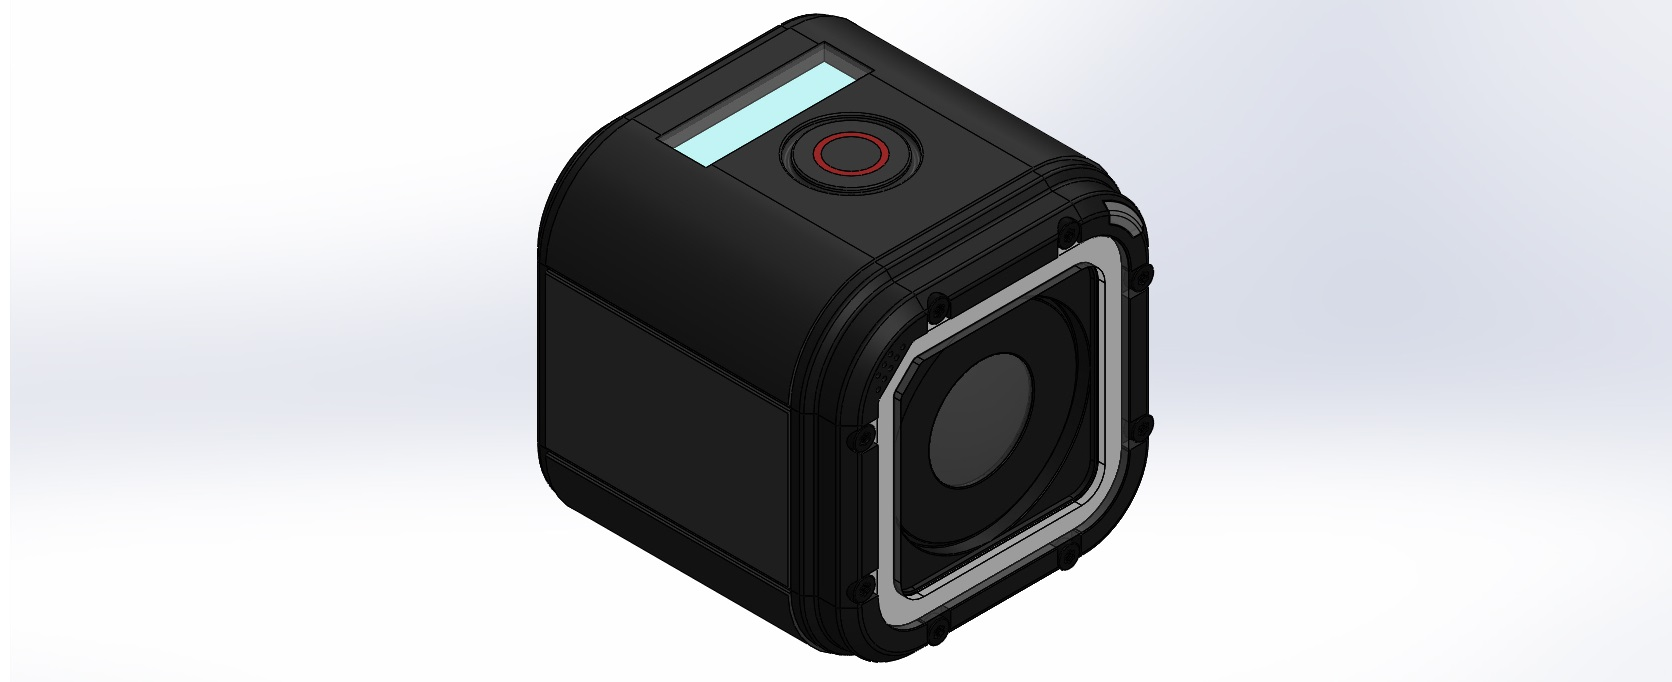
\includegraphics[width=0.9\linewidth]{figures/GoProHero4Session.JPG}
\caption{3D CAD rendering of the GoPro Hero Session action camera from \cite{gph4smodelgrabcad}}
\label{fig:GoProHero4Session}
\end{figure}

The camera can capture videos at a variety of frame rates and a variety of resolutions. These settings are limited as the software that controls the camera is proprietary. The set frame rates and resolutions are presented in the table below.

\begin{table}[!ht]
\centering
\captionsetup{width=0.8\linewidth, font=small}  
\caption{Possible frame rate and resolution combinations on the GPHS camera}
\label{framesres}
\begin{tabular}{ll}
Resolution  & Frame Rates                             \\
1920 x 1440 & 30 fps, 25 fps                          \\
1920 x 1080 & 60 fps, 50 fps, 48 fps, 30 fps, 25 fps  \\
1280 x 960  & 60 fps, 50 fps, 30 fps, 25 fps          \\
1280 x 720  & 100 fps, 60 fps, 50 fps, 30 fps, 25 fps \\
848 x 480   & 120 fps, 100 fps                       
\end{tabular}
\end{table}

The relative motion of the lower limbs appeared to move rapidly when viewing test footage and therefore the highest possible frame rate with the best resolution was chosen. The camera was configured to record at 100Hz and at a resolution of 1280 x 720 pixels. This was chosen as the quality of the 848 x 480 video was assumed to distorted to identify the marker centres with computer algorithms.

The camera also has the ability to record using a normal lens or a wide angle lens. The field of view of the camera greatly increases with the wide angle lens but its focal length decreases proportionally. The wide lens also produces more distortion when compared to the normal lens. \cite{Hartley2004}. Due to the relatively narrow area of capture needed the camera was configured to use the normal lens as it would decrease distortion without compromising the area of interest.

Naturally, working with proprietary hardware presents some difficulties. One of these difficulties is created by the GoPro camera regulating its exposure automatically. In darker environments the GoPro will automatically change to low light mode, causing inconsistent light levels in videos taken in different conditions. This causes uncertainty when trying to use feature detection since the varying light levels change the relative colors of the markers.

Another difficulty is the output video files generated by the GoPro. These files have a .MP4 file extension implying that they have already been compressed. This compression causes a loss of precision opposed to the raw video data being recorded. Compression had been implemented to save memory on the GoPro's micro SD memory card. Decompressing this video data will be discussed in the following chapter.

\section{Camera Mount Design}
Some initial work on modelling a housing for the camera was completed by the Mechatronics Research Lab. This was a 2 part 3D printable enclosure with no mounting points or control access. The enclosure is pictured below.

\begin{figure}[!ht] 
\captionsetup{width=0.8\linewidth, font=small}  
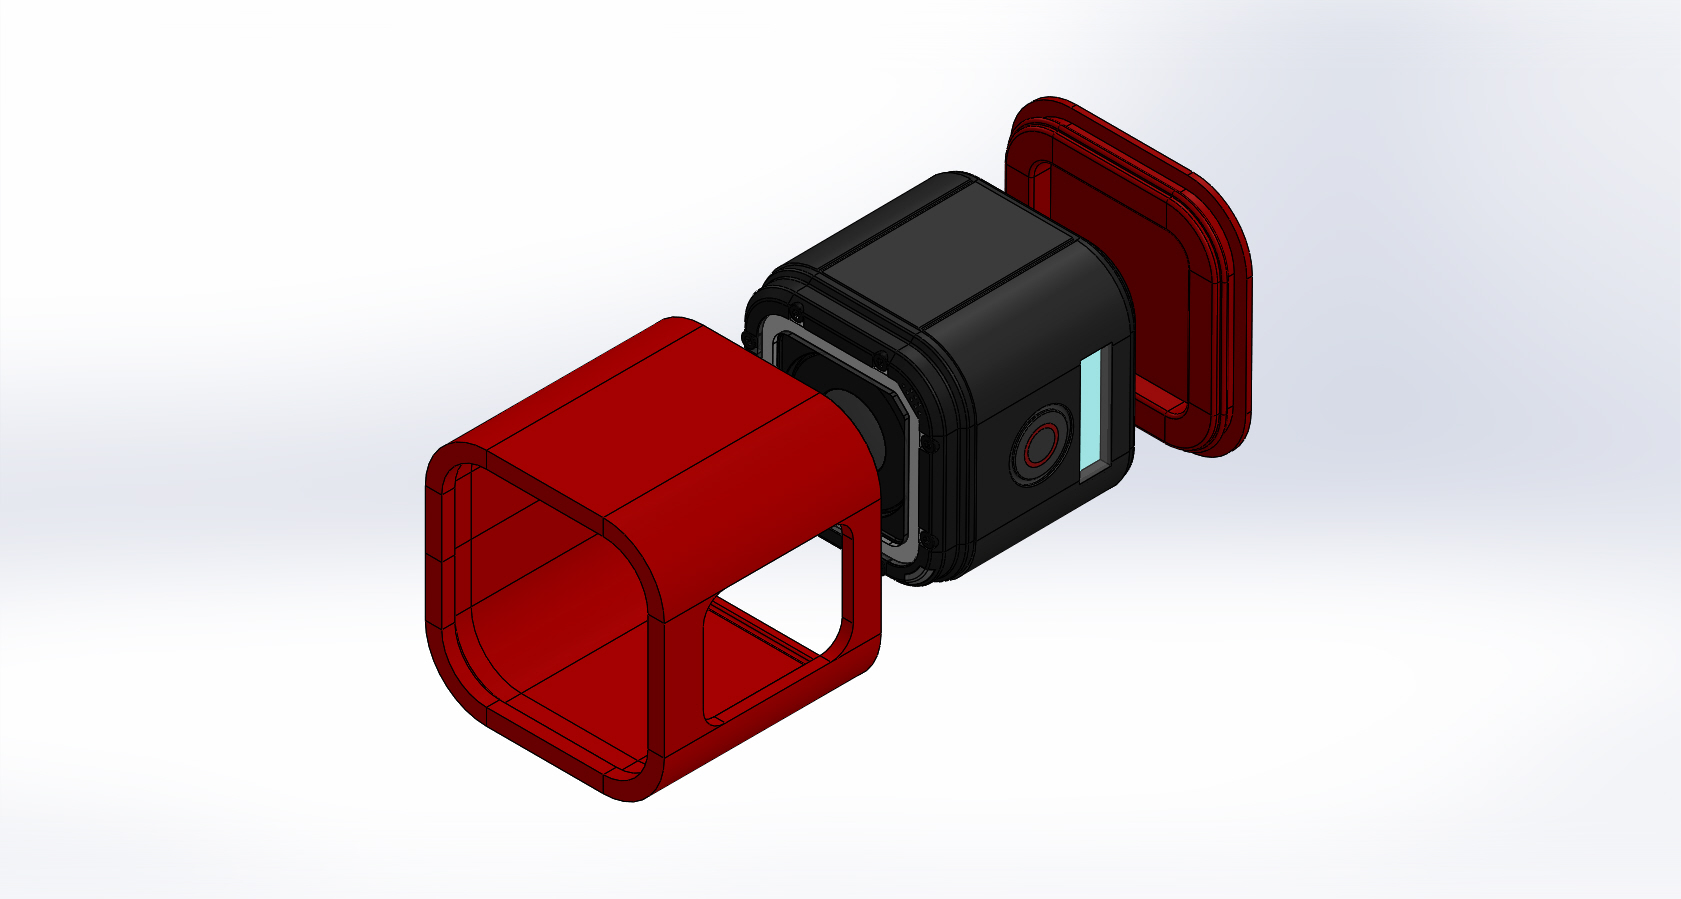
\includegraphics[width=0.6\linewidth]{figures/sylvanexploded.JPG}
\caption{Initial camera enclosure designed by the mechatronics lab}
\label{fig:sylvanexploded}
\end{figure}

This model was heavily modified using Dassault Systems SOLIDWORKS software to enclose 2 cameras mounted side by side. The bracket also needed a mounting point to join to the chest mount. Finally the bracket needed to be lightweight, provide access to the camera controls and not obscure the built in status screen of the cameras. The following figure shows the final dual camera bracket that was 3D printed. This bracket can be found on the accompanying CD.

\begin{figure}[!ht] 
\captionsetup{width=0.8\linewidth, font=small}  
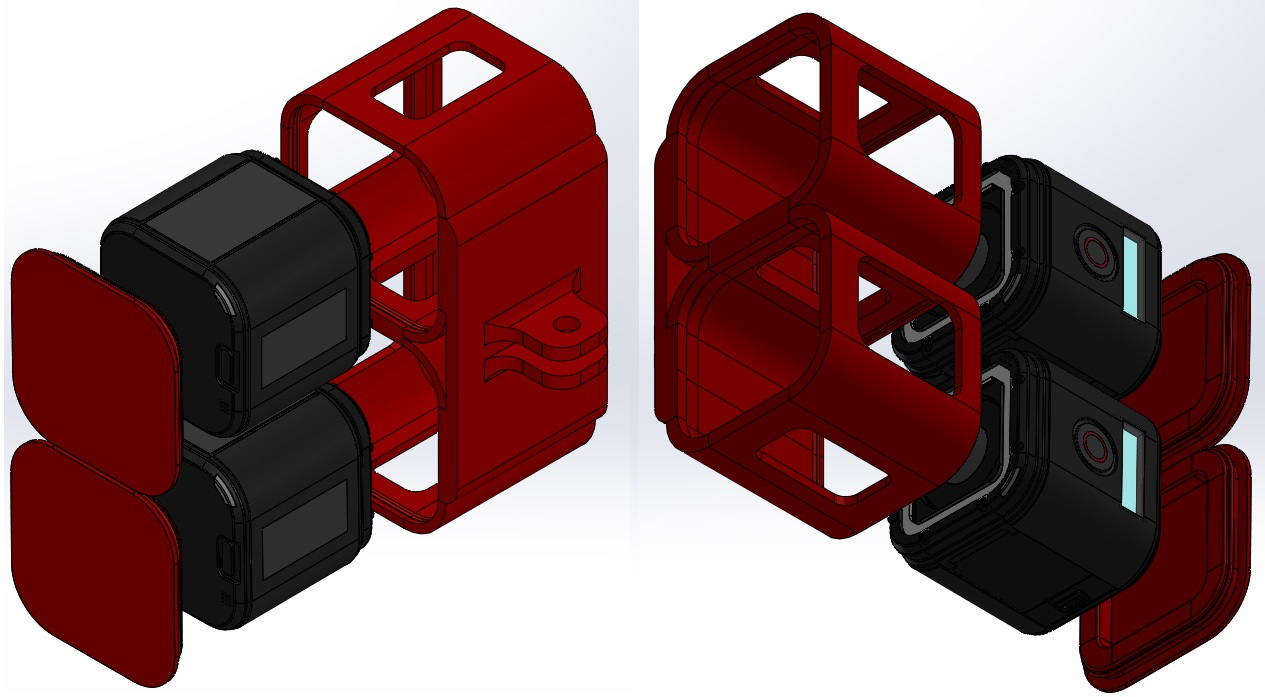
\includegraphics[width=0.6\linewidth]{figures/stereoholder.JPG}
\caption{Final dual camera enclosure designed by the author}
\label{fig:stereoholder}
\end{figure}

As seen in the figure above the sides of the housing was opened to reduce the overall weight of the mount. These opening also serve as access to the controls and status screen on the GoPros. The mounting piece of the housing was designed to mate with standard GoPro screw connectors allowing it to be used on a variety of GoPro harnesses. 

This bracket was mounted to the Action Mounts Chest mount. One bracket was mounted to the front of the chest mount and using the included GoPro mounting pads the chest harness was modified to carry a bracket on the back plate as well. The back plate of the Chest Harness was relatively small and when examining the footage taken during test runs the rear camera pair was found to be very unstable. The following diagram shows the chest harness.

\begin{figure}[!ht] 
\captionsetup{width=0.8\linewidth, font=small}  
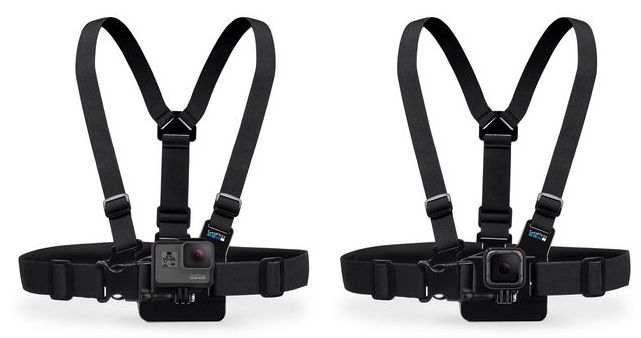
\includegraphics[width=0.6\linewidth]{figures/chesty.png}
\caption{Action Mounts chest mount showing the front mounting plate}
\label{fig:chesty}
\end{figure}

The need to increase the stability without hindering wearability introduced a new specification to be incorporated into the design process. The part had to comfortably fit to the back of a runner while providing a larger surface area for the camera to mount too. The part shown in the following figure was created and tested to fulfil this specification.

\begin{figure}[!ht] 
\captionsetup{width=0.8\linewidth, font=small}  
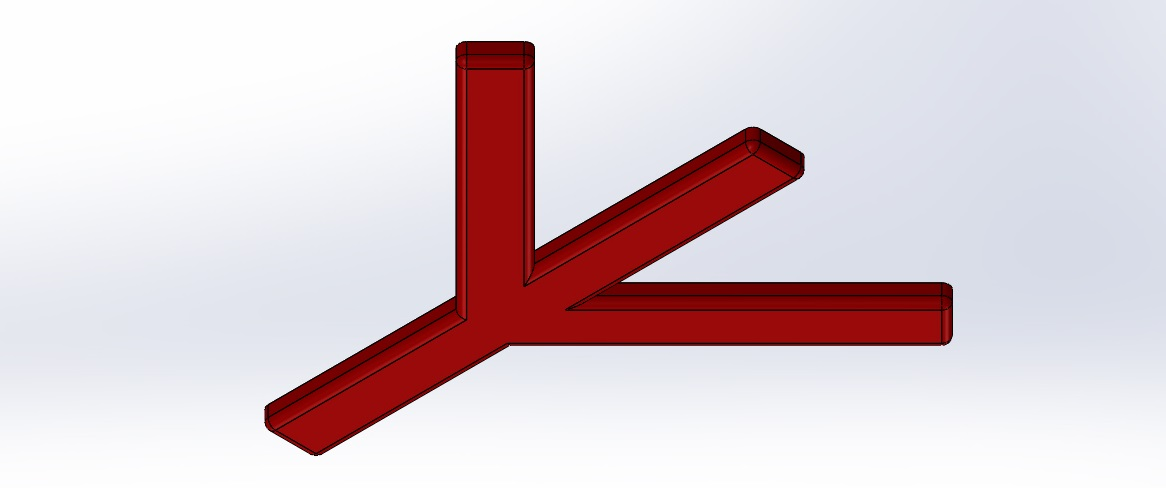
\includegraphics[width=1\linewidth]{figures/stabil.JPG}
\caption{Stabilizer mounted to the rear camera}
\label{fig:stabil}
\end{figure}

The stabilizer was fastened to the back of the harness backplate. The following figure shows stabilizer mounted below the rear camera.

\begin{figure}[!ht] 
\captionsetup{width=0.8\linewidth, font=small}  
\includegraphics[width=0.8\linewidth]{figures/pats.png}
\caption{Stabilizer mounted to the rear camera}
\label{fig:pats}
\end{figure}

When comparing footage of the back cameras before and after the stabilizer was attached a clear difference is noted. The videos before contained excessive movement to the extent that the image blurred the lower limbs. This would prove problematic for attempts at image processing as the relatively low resolution and blurry images would introduce large uncertainties in the marker locations. After interviewing subjects wearing the data capture system did not reduce the comfortability of the system. 


\section{Sony Xperia Z3 Compact Smartphone}
The Sony Xperia Z3 Compact has a complex sensor system that includes an accelerometer, gyroscope, magnetometer, light sensor, pressure sensor, and proximity sensor. These sensors are combined locally to also create artificial sensors for orientation, gravity, and linear acceleration. A built in GPS is also available to provide positional data. These sensors are updated constantly and pushed to different memory locations as explained in the Android API documentation. 

To log the different datapoints generated by the sensors a software application for the smartphone was needed. Many free applications are available on the Android Marketplace to fulfil this purpose; largely due to the open source approach the Android operating system is built on. By checking user reviews and ratings the following applications were considered.

\subsection{AndroSensor}
Androsensor was created by Fiv Asim and is availible freely from the Android marketplace or \cite{androsensor}. The source code for this application is not available, but the author details the various underlying methods on \cite{androsensor}. The following are screenshots of the application running on the Z3 Compact.

\begin{figure}[!ht] 
\captionsetup{width=0.8\linewidth, font=small}  
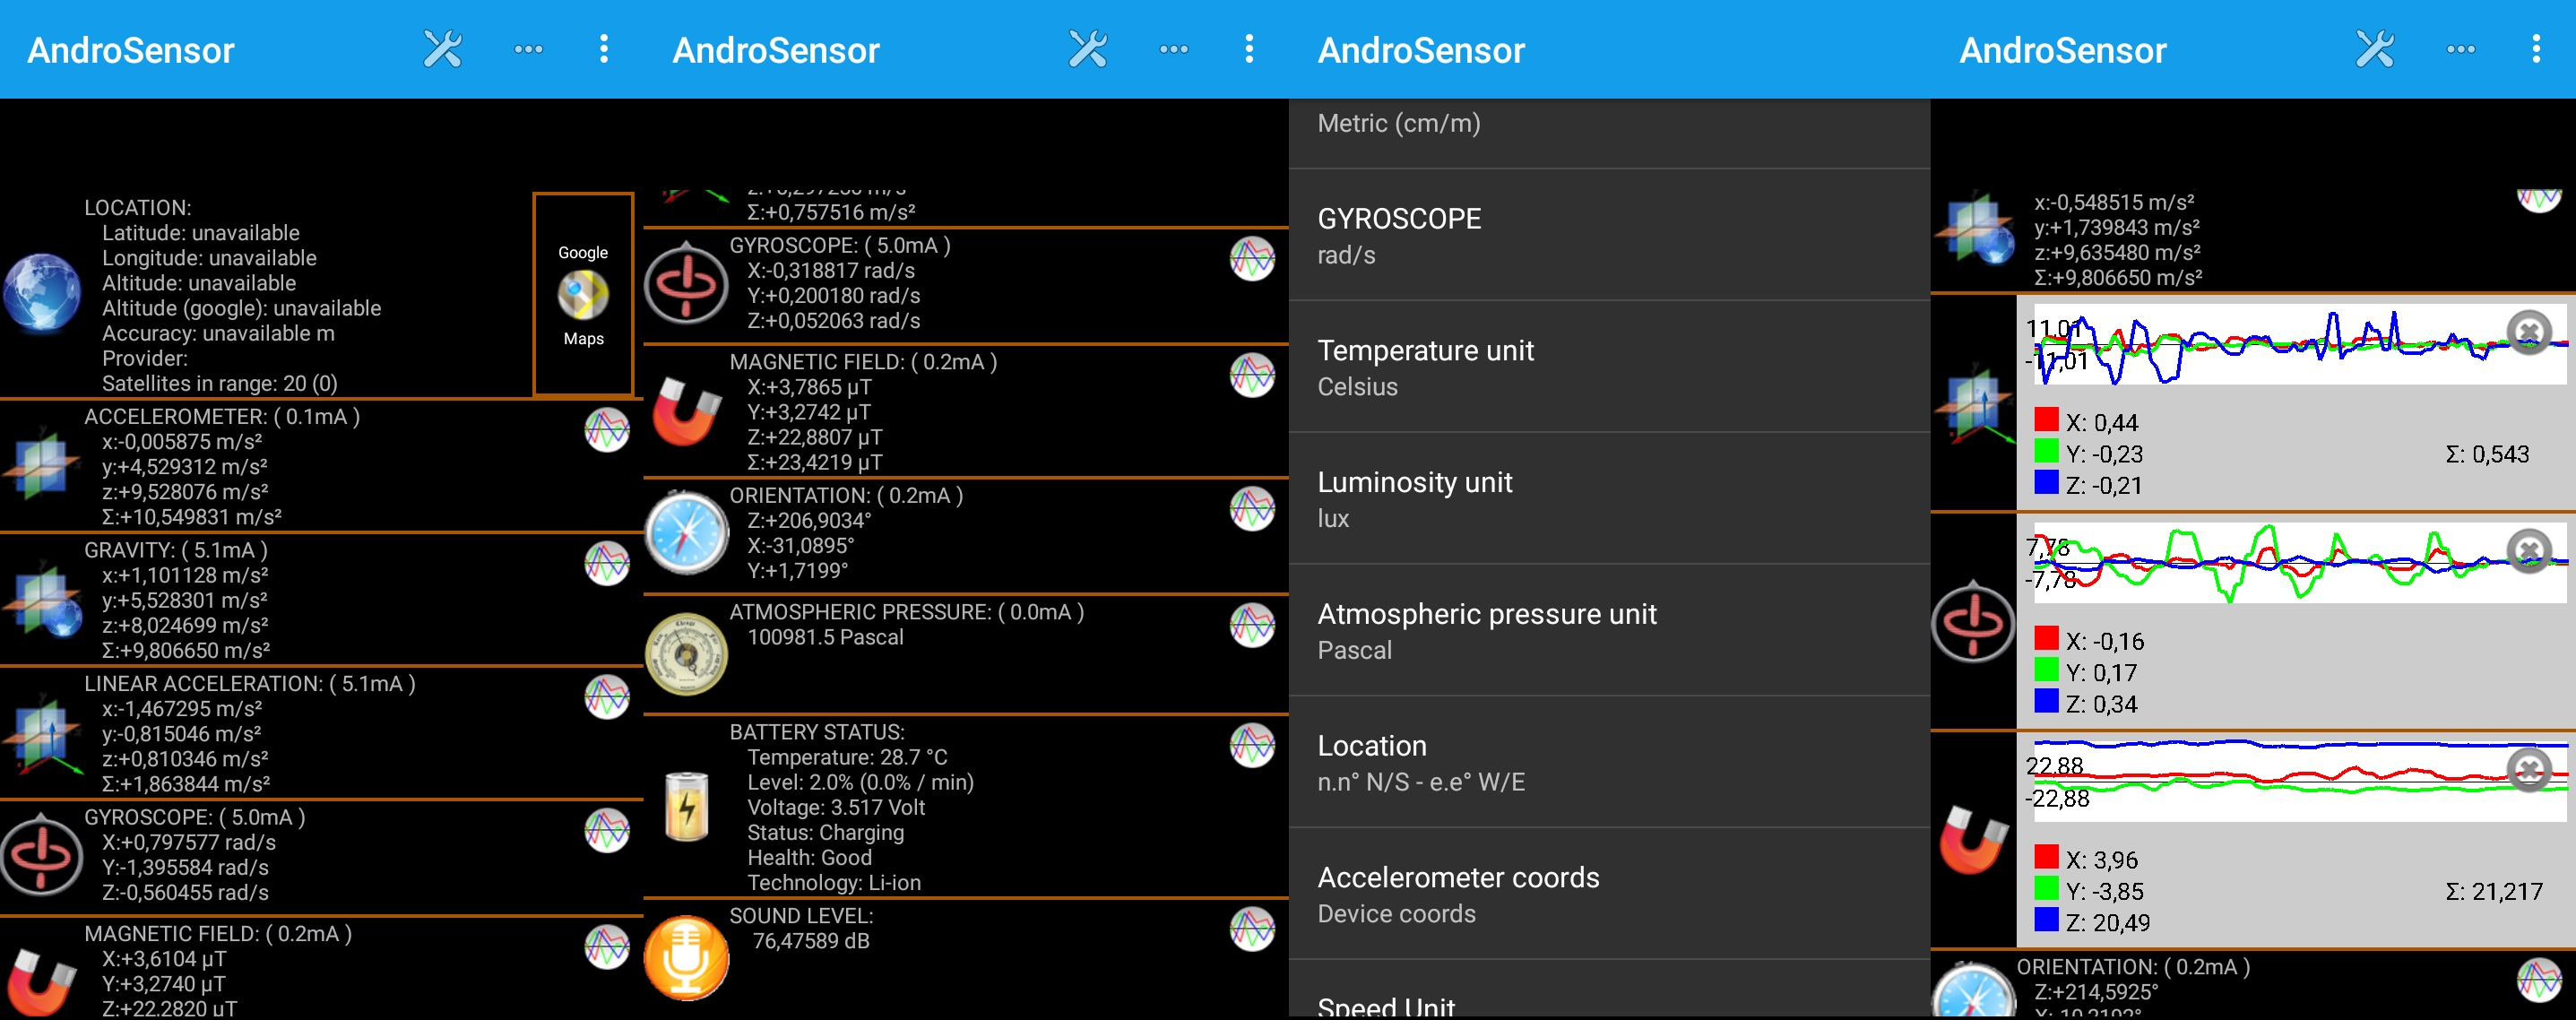
\includegraphics[width=0.8\linewidth]{figures/screeniesas.jpg}
\caption{AndroSensor mobile application running on the Sony Xperia Z3 Compact}
\label{fig:screeniesas}
\end{figure}

One of the advantages of AndroSensor is that it is highly configurable. A user can select which sensors are monitored and logged and the rate at which they are updated. This allows us to log important data and eases pre processing efforts. The application can also log the magnitude of sound allowing us to use this to synchronize the entire system. The output file type and units of the sensors can also be configured also easing pre processing. 

There is a drawback to not being able to view the source code of the application, we can not be sure if the data the application provides is raw real time data or filtered delayed data. This could introduce a delay to the system causing desynchronization of the different data sources.

\subsection{SensorLab}
Another popular application is SensorLab, created by LP Allis and available freely on the Google Play Store. This application is newer that AndroSensor and based on a more recent version of the Android APK. This should allow the application to run more efficiently and log data faster and more accurately. The following are screenshots taken from within SensorLab.

\begin{figure}[!ht] 
\captionsetup{width=0.8\linewidth, font=small}  
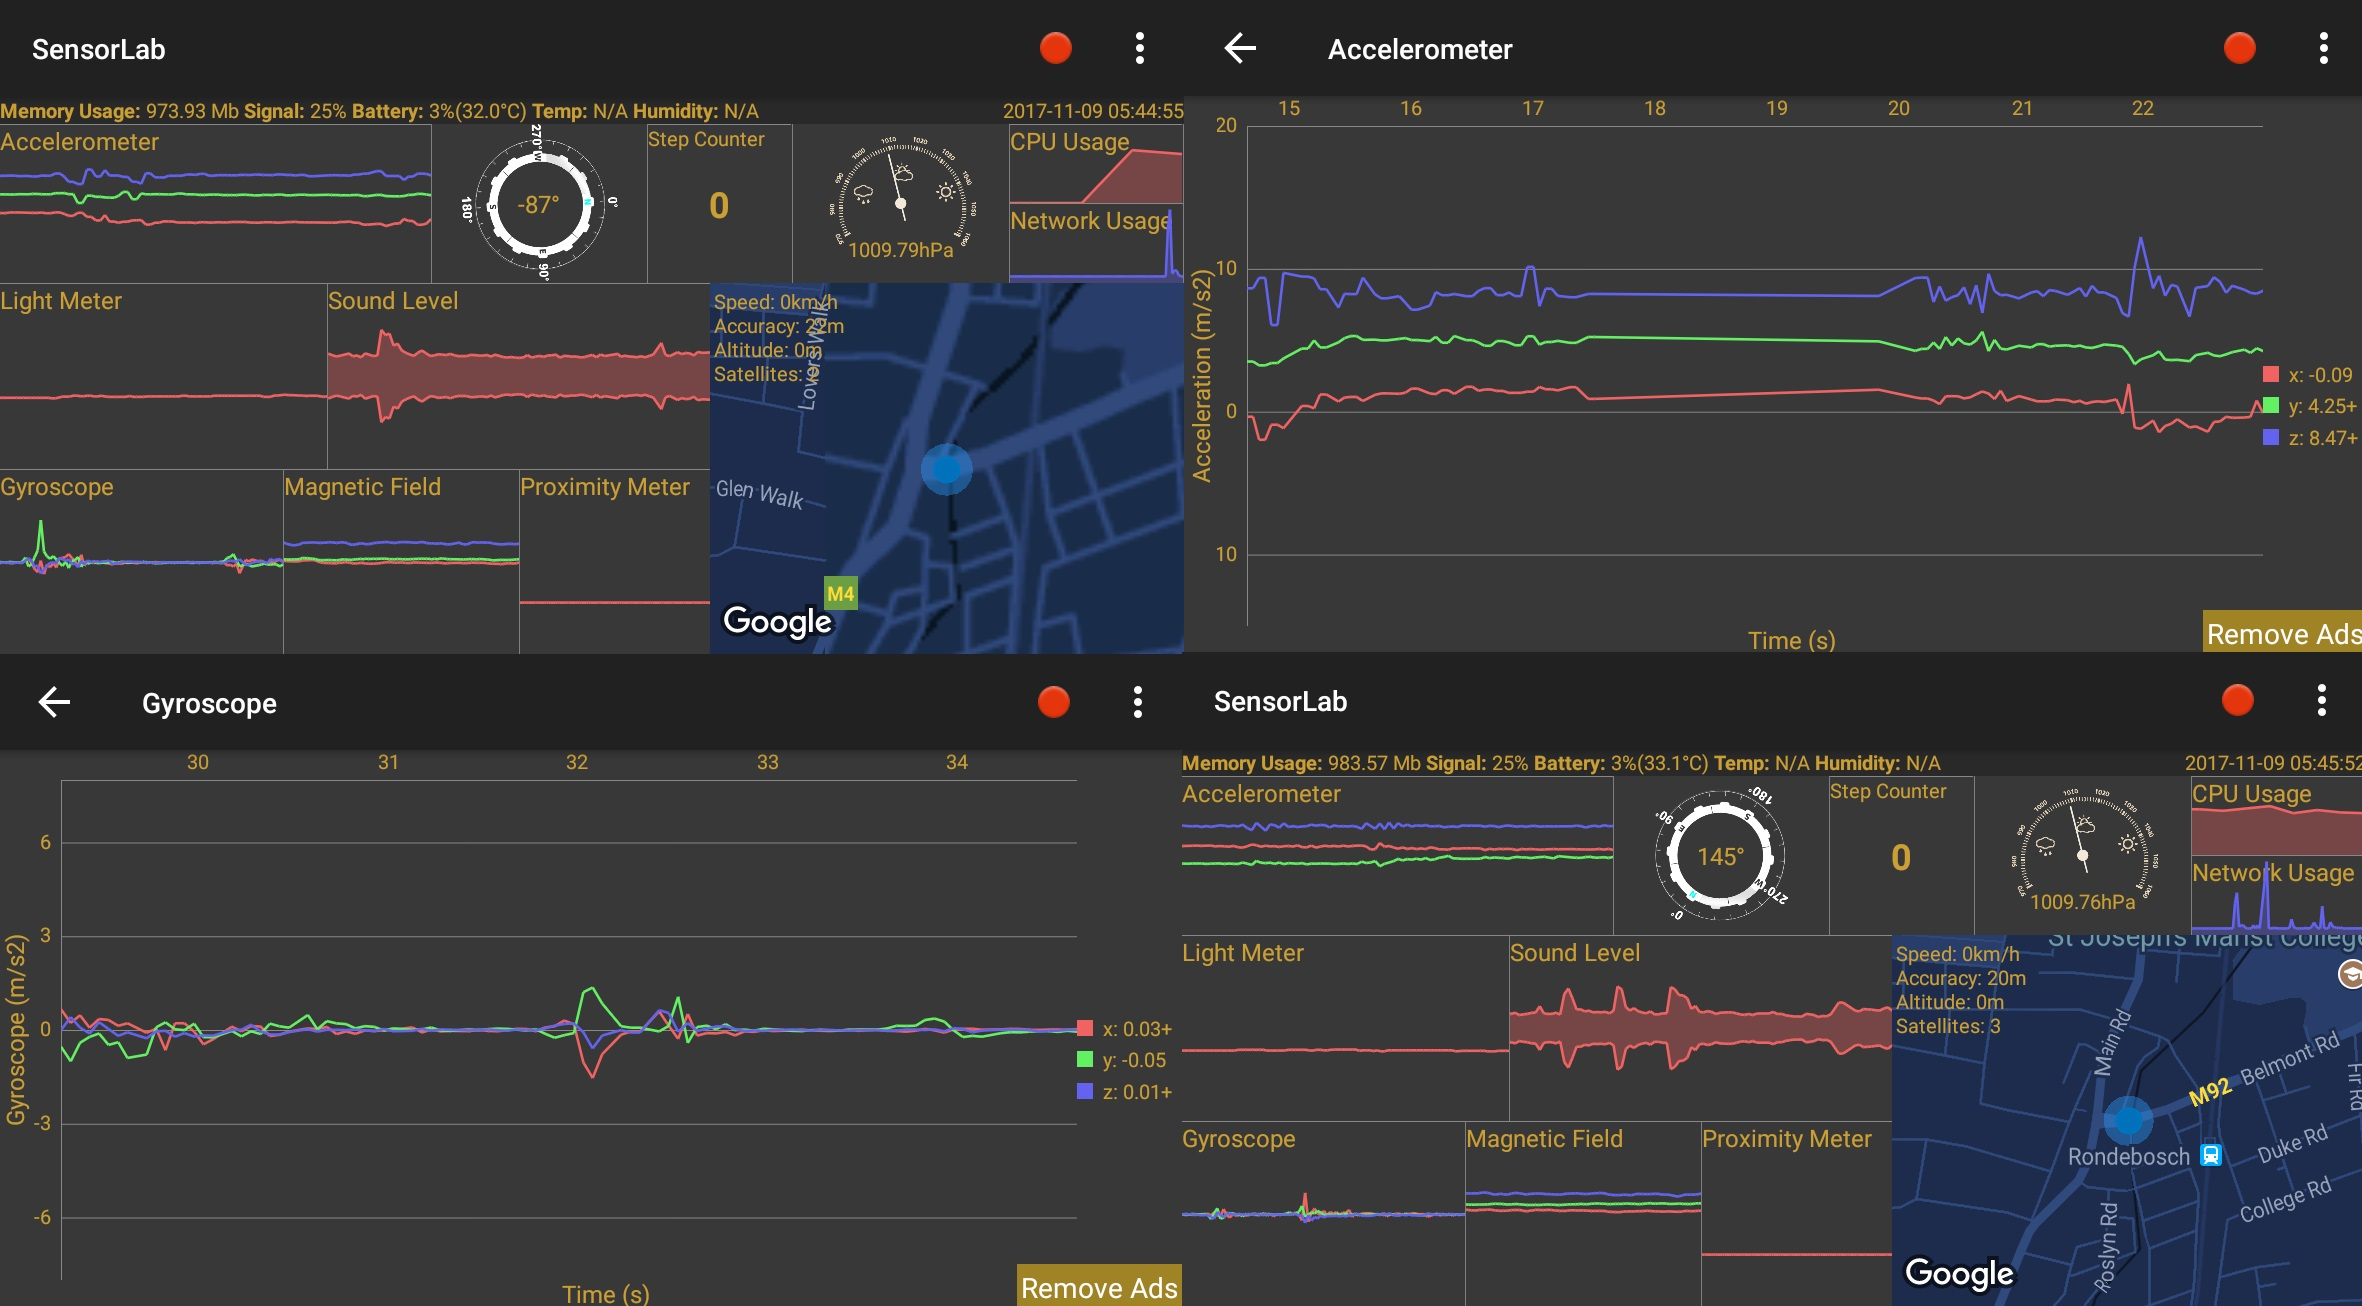
\includegraphics[width=0.8\linewidth]{figures/sls.jpg}
\caption{SensorLab mobile application running on the Sony Xperia Z3 Compact}
\label{fig:screeniessl}
\end{figure}

This application has very little configurability. It automatically logs all sensor data at the maximum possible rate. After analysing the output file generated by SensorLab the logging rate was found to be 150Hz for most sensors. The parameters logged however did not include a volume reading, introducing synchronization difficulties.

The application is also closed source, making it impossible to know if the data values are processed or not. It was also unclear what units some of the data values were logged in, increasing the complexity of pre processing the data.

\subsection{Custom Software}
A custom software solution was developed by Stocks in \cite{bradstocks} to log the various sensors of the smartphone. This application was developed to include readings from external sensors as well as the internal sensors of the smartphone. The source code for the application is available and  

\begin{figure}[!ht] 
\captionsetup{width=0.8\linewidth, font=small}  
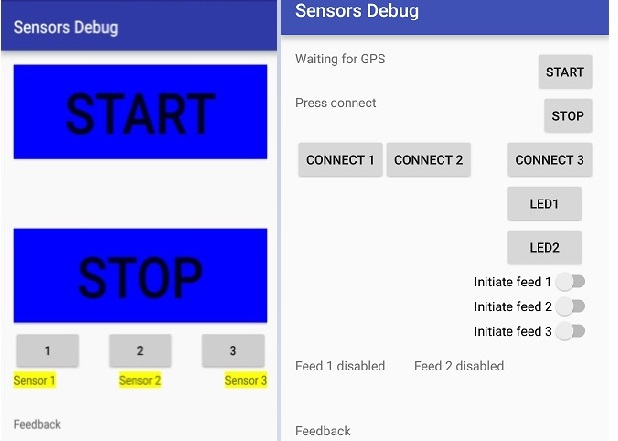
\includegraphics[width=0.4\linewidth]{figures/bradbadcode.jpg}
\caption{Stabilizer mounted to the rear camera}
\label{fig:bradbadcode}
\end{figure}

When the source code of the application was compiled using android studio the application did not function. The source code provided was not the final source code used for the research project. An attempt was made to modify the source code to correct the application but proved impossible due to the large codebase and lack of documentation.

\subsection{Final Selection}
AndroSensor was selected over the over application due to the above mentioned advantages. The application was configured to log the accelerometer, gyroscope, magnetometer, GPS location, and sound level. The logging rate was set at 100Hz to have uniformity in the system. Once the data was logged the output file contained the following headings. 

\begin{table}
\centering
\captionsetup{width=0.8\linewidth, font=small}  
\caption{This table shows the different headings of the output AndroSensor file}
\label{Smartphone Data Headings}
\begin{tabular}{ll}
Heading               & Fields  \\
ACCELEROMETER       & X,Y,Z  \\
GRAVITY              & X,Y,Z \\
LINEAR ACCELERATION  & X,Y,Z\\
GYROSCOPE            & X,Y,Z \\
MAGNETIC FIELD       &  X,Y,Z\\
ORIENTATION          &  X,Y,Z\\
ATMOSPHERIC PRESSURE  &      \\
LOCATION Latitude     &       \\
LOCATION Longitude    &       \\
LOCATION Speed        &       \\
LOCATION ORIENTATION  &       \\
VOLUME
\end{tabular}
\end{table}


\section{Smartphone Mount Design}
The design specification was to rigidly mount the smart phone to the chest of the subject. To complete this objective a rubber smartphone housing for the Z3 compact was fastened to the ActionMounts chest mount above the front duel camera. The following image illustrates the smartphone as connected to the harness. If the smartphone had been mounted on top of the camera we could have used pose estimation to understand exactly the orientation of the camera with respect to the world frame.

\begin{figure}[!ht] 
\captionsetup{width=0.8\linewidth, font=small}  
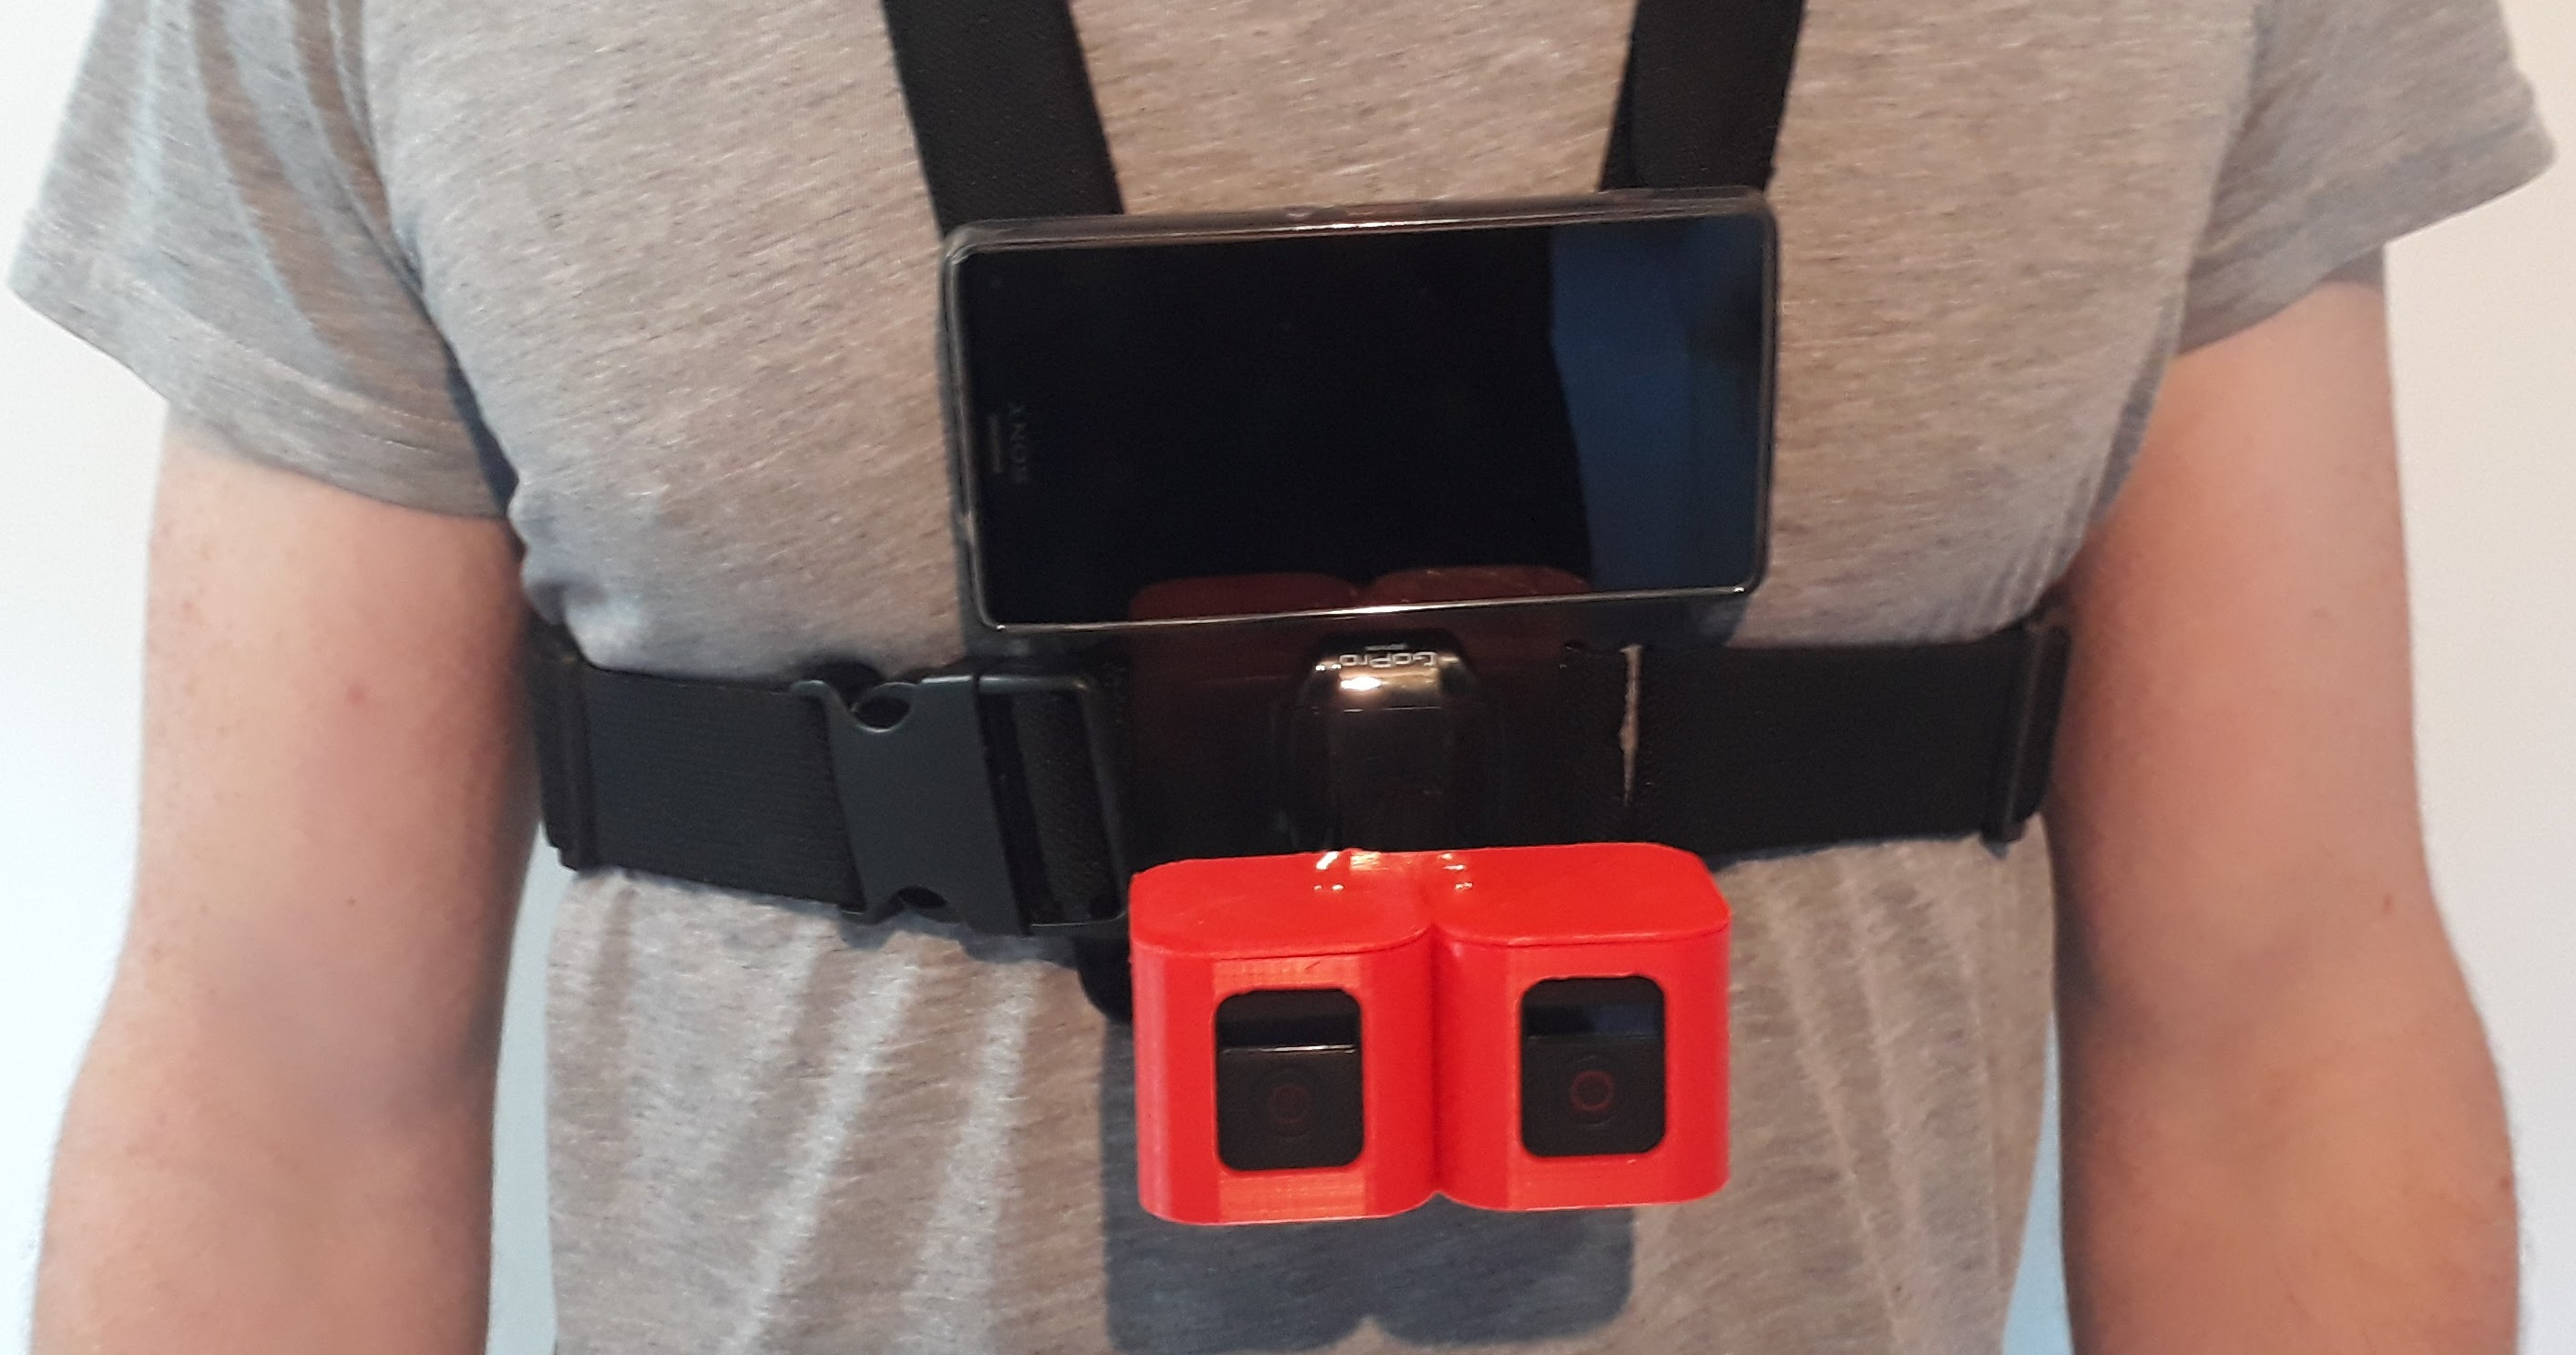
\includegraphics[width=0.6\linewidth]{figures/pm.JPG}
\caption{phone mount}
\label{fig:pm}
\end{figure}

\section{Critical Point Markers}
To increase the accuracy of the image processing elements of this methodology various colourful markers were used to identify critical points on the subjects lower extremities. The following picture shows the location of the markers.

\begin{figure}[!ht] 
\captionsetup{width=0.8\linewidth, font=small}  
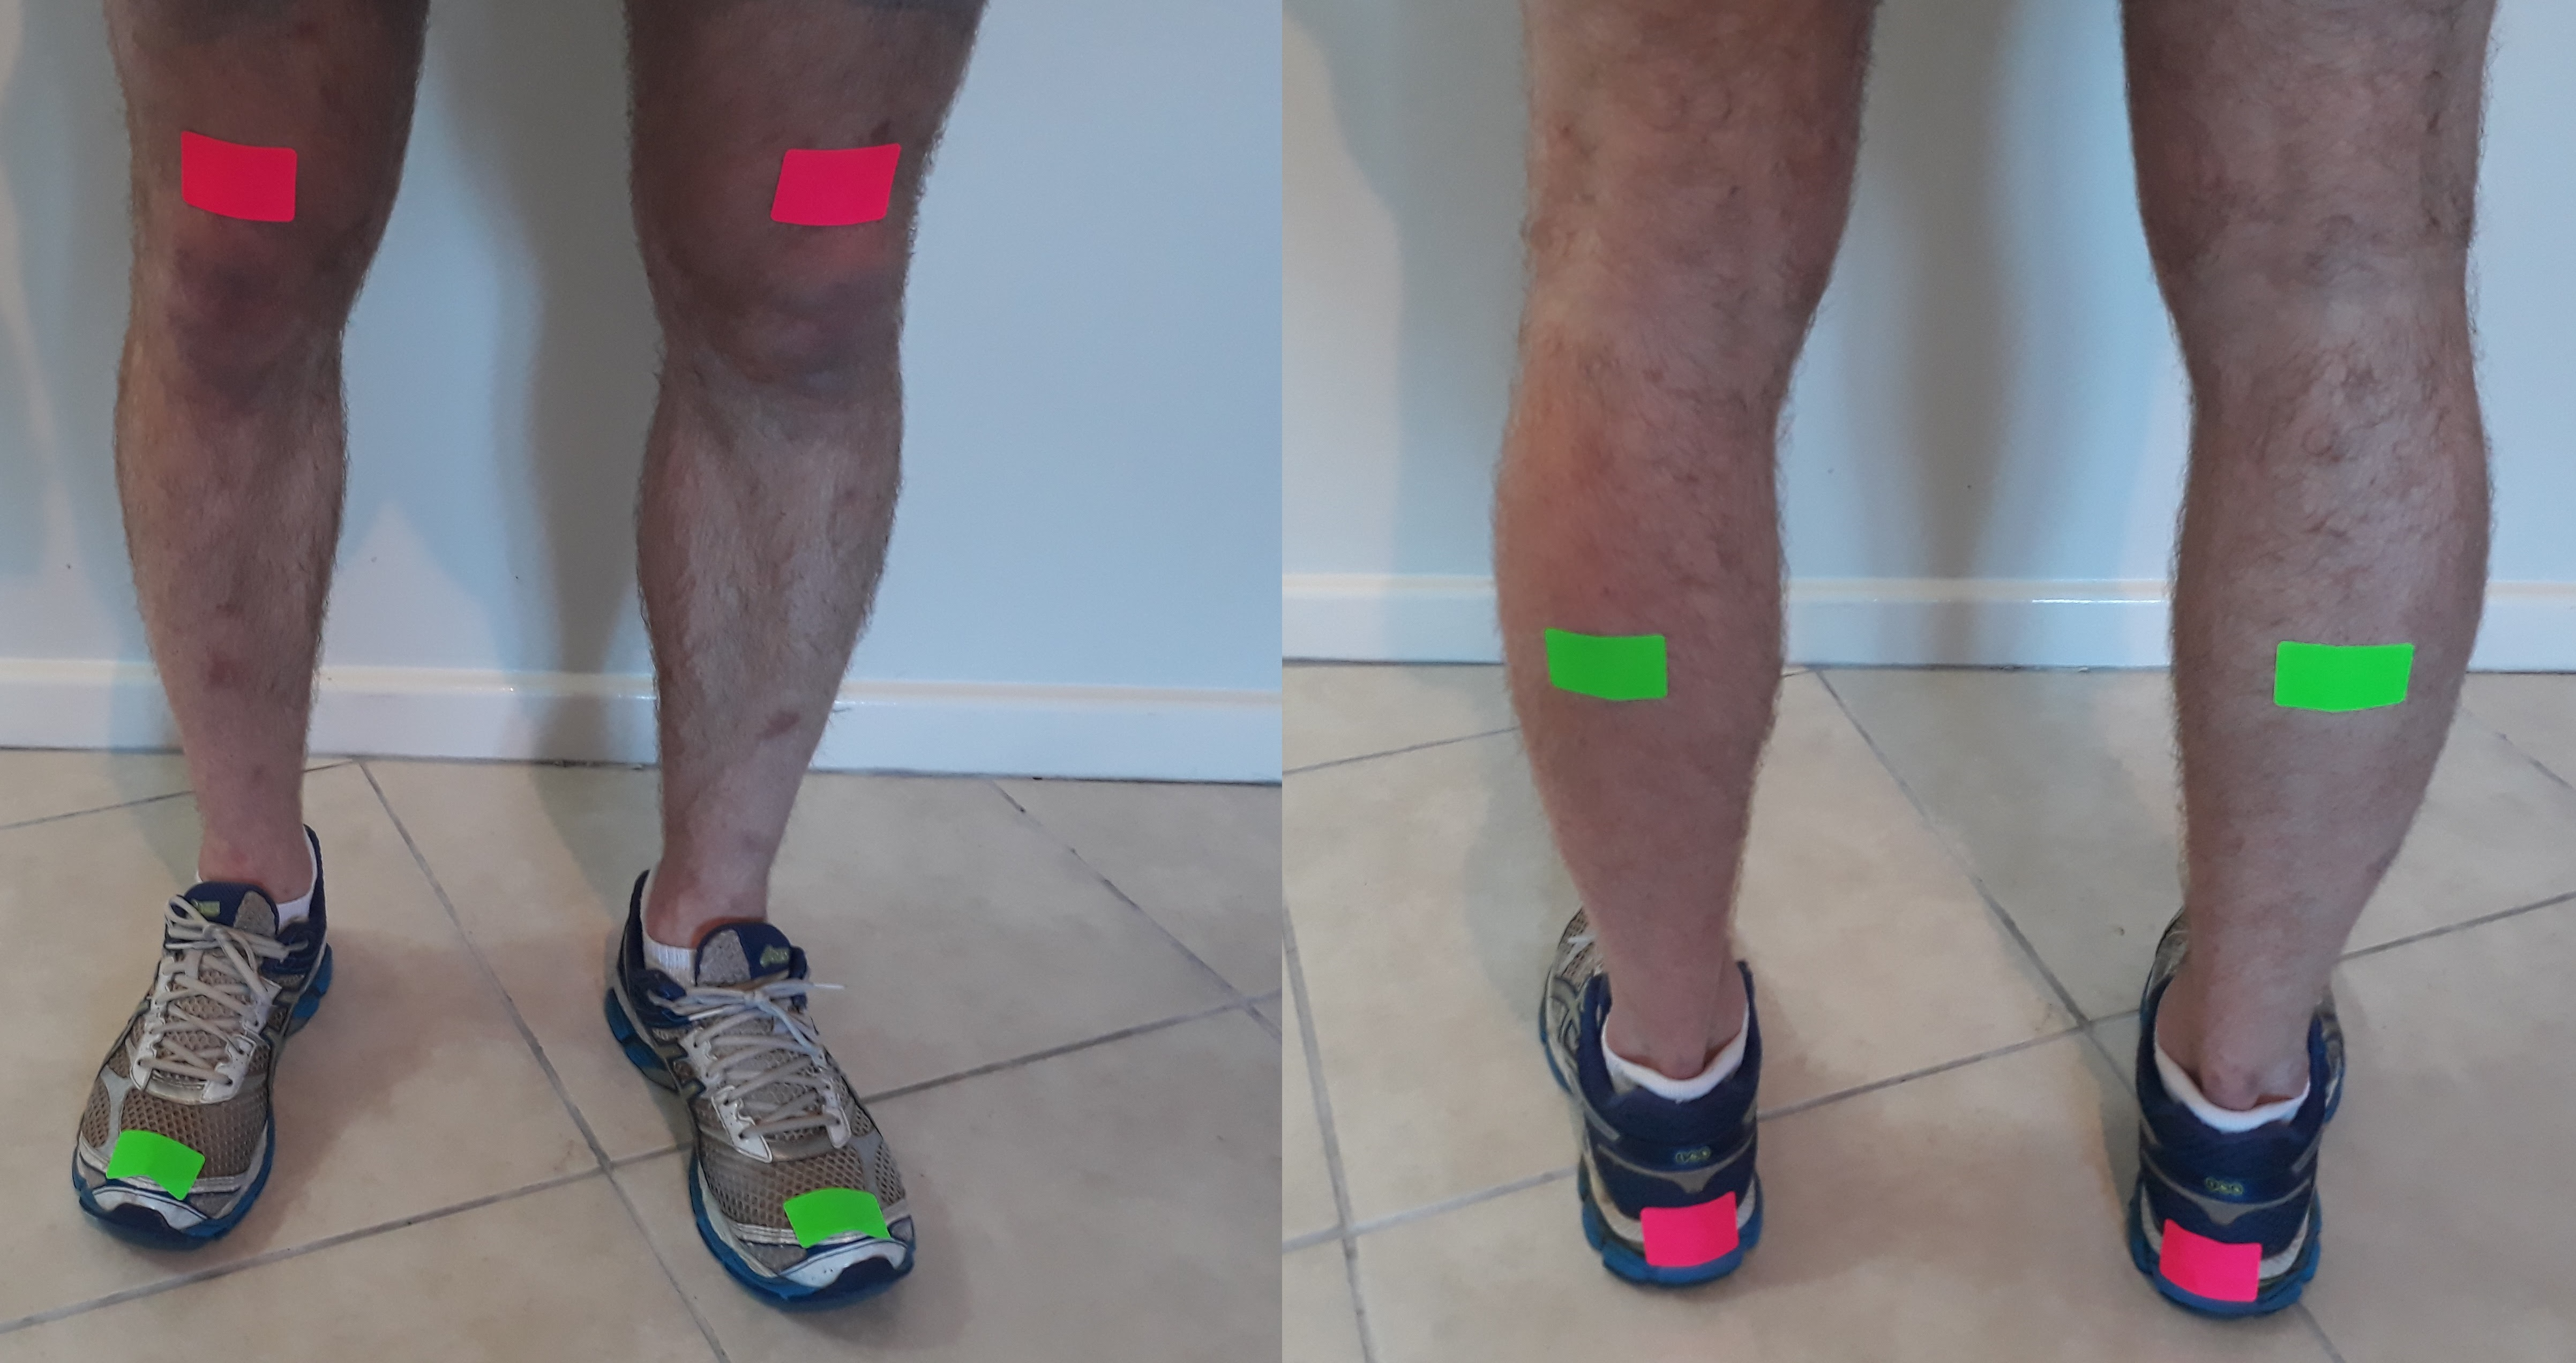
\includegraphics[width=\linewidth]{figures/markers.JPG}
\caption{Subject wearing Green and Pink Markers to identify critical points}
\label{fig:markers}
\end{figure}

From the image we can see that green markers were used to identify  the toe edge of the runner in the front camera frame and pinks marker to identify the end of the thigh in the same frame. In the rear mounted camera frame pink markers were used to identify the heel of the subject and green markers to identify the centre of the calf. These markers in conjunction with the model is used to identify the lower limb orientation during the fusion stage.

These luminous green and pink markers were chosen because they are bright in most lighting conditions and offer a stark contrast to both the subjects clothing and skin colour. They also contrast a typical black tar road surface where the runs were performed. This contrast makes them easy to detect using feature detection as they  cause a spike in the color decomposition of the image.




